%%%%%%%%%%%%%%%%%%%%%%%%%%%%%%%%%%%%%%%%%
% Programming/Coding Assignment
% LaTeX Template
%
% This template has been downloaded from:
% http://www.latextemplates.com
%
% Original author:
% Ted Pavlic (http://www.tedpavlic.com)
%
% Note:
% The \lipsum[#] commands throughout this template generate dummy text
% to fill the template out. These commands should all be removed when 
% writing assignment content.
%
% This template uses a Perl script as an example snippet of code, most other
% languages are also usable. Configure them in the "CODE INCLUSION 
% CONFIGURATION" section.
%
%%%%%%%%%%%%%%%%%%%%%%%%%%%%%%%%%%%%%%%%%

%----------------------------------------------------------------------------------------
% PACKAGES AND OTHER DOCUMENT CONFIGURATIONS
%----------------------------------------------------------------------------------------

\documentclass{scrartcl}

\usepackage{fancyhdr} % Required for custom headers
\usepackage{extramarks} % Required for headers and footers
\usepackage[usenames,dvipsnames]{color} % Required for custom colors
\usepackage{graphicx} % Required to insert images
\usepackage{listings} % Required for insertion of code
\usepackage{courier} % Required for the courier font
\usepackage{lmodern}
\usepackage{media9}
\usepackage[hidelinks]{hyperref}
\usepackage{wrapfig}
\usepackage{listing}
\usepackage{xcolor}
\usepackage{media9}

\usepackage[square]{natbib}
\usepackage{dblfloatfix}
\usepackage{fixltx2e}

\usepackage[T1]{fontenc} % placer ici votre encodage préféré
\usepackage[utf8]{inputenc} % placer ici votre encodage préféré
\usepackage{amsmath}
\usepackage{parskip}
\newcommand{\HRule}{\rule{\linewidth}{0.5mm}}

\graphicspath{ {res/} }

% Margins
\topmargin=-0.45in
\evensidemargin=0in
\oddsidemargin=0in
\textwidth=6.5in
\textheight=9.0in
\headsep=0.25in

\linespread{1.1} % Line spacing

% Set up the header and footer
\pagestyle{fancy}
\rhead{\firstxmark} % Top right header
\lfoot{\lastxmark} % Bottom left footer
\cfoot{} % Bottom center footer
\rfoot{Page\ \thepage} 
\renewcommand\headrulewidth{0.4pt} % Size of the header rule
\renewcommand\footrulewidth{0.4pt} % Size of the footer rule

\setlength\parindent{0pt} % Removes all indentation from paragraphs


%----------------------------------------------------------------------------------------
% DOCUMENT STRUCTURE COMMANDS
% Skip this unless you know what you're doing
%----------------------------------------------------------------------------------------

% Header and footer for when a page split occurs within a problem environment
\newcommand{\enterProblemHeader}[1]{
\nobreak\extramarks{#1}{#1 continued on next page\ldots}\nobreak
\nobreak\extramarks{#1 (continued)}{#1 continued on next page\ldots}\nobreak
}

% Header and footer for when a page split occurs between problem environments
\newcommand{\exitProblemHeader}[1]{
\nobreak\extramarks{#1 (continued)}{#1 continued on next page\ldots}\nobreak
\nobreak\extramarks{#1}{}\nobreak
}

\lstdefinestyle{sharpc}{language=[Sharp]C, frame=lr, rulecolor=\color{blue!80!black}}
\begin{document}


\lstset{style=sharpc}
%----------------------------------------------------------------------------------------
% TITLE PAGE
%----------------------------------------------------------------------------------------

\begin{titlepage}
\begin{center}

% Upper part of the page. The '~' is needed because \\
% only works if a paragraph has started.

\textsc{ Kungliga Tekniska Högskolan \\ School of Computer Science and Communication}\\[1.5cm]

\begin{figure}[ht]
\begin{center}

\includegraphics[width=0.65\textwidth]{KTH}
\end{center}
\end{figure}

\textsc{\Large DH2323}\\[0.5cm]

% Title
\HRule \\[0.4cm]
 { \huge \bfseries Citibike Bicycle Traffic Visualization \\[0.4cm] }
{\large \bfseries  Project Documentation\\[0.4cm] }

\HRule \\[1.5cm]

% Author and supervisor
\begin{minipage}{0.65\textwidth}
\begin{flushleft} \large
Michael \textsc{Hotan} PN: 870522-T599 SN: 0579 5268\\
Alexandre \textsc{St-Onge}\\
\end{flushleft}
\end{minipage}

\vfill

% Bottom of the page
{\large \today}

\end{center} 
\end{titlepage}

%----------------------------------------------------------------------------------------
% Introduction
%----------------------------------------------------------------------------------------

\section{Introduction}

The prominence of utilizing real time sensor data to create powerful visualization has broadened uses of Computer Graphics.  We were inspired by the availability of Citibike's bicycle sharing system data. bicycle transportation data provided by and.  New York City, like many other populated cities, set up a bicycle sharing system.  A benefit in having such a system is that it allows an intrinsic way to store traffic data.  We looked to build a Unity application that depicts a bicycle scene in which traffic density reflects Citibike data.

\section{Background}

Citibike and New York City opened up their trip data set allowing computer scientists, data enthusiasts, and analysts to create powerful visualizations.  \citep{Citibike:Visualization} shows how traffic trends over 48 hours using a two dimensional map.  We attempted to build on concepts presented in \citep{peters2011crowds} except in a bicyclist context.  We wanted to create a realistic bicycle traffic visualization that could represent the varying levels of traffic density found within Citibike's dataset.  This included 5 essential tasks: 

\begin{enumerate}
  \item Create a background scene.
  \item Simulate bike traffic.
  \item Write custom shaders.
  \item Create controls for augmenting displayed bike traffic.
  \item Connect and augment the visualization in accordance to New York Citibike data. 
\end{enumerate}

I was involved with parts 3, 4, and 5.  I will provide an overview for each task but only go into detail in the parts I implemented.  We ended up using Blender to edit our models and Unity to create our visual scene, manage animations, and write our shaders and scripts.
	
\section{Process}

In order to facilitate our lack of experience in modelling three dimensional objects, we decided to implement a top down approach for this project.  We used predefined Unity Assets for our scene and cyclist model.  The cyclist model, created by \citep{Bicycle:Blender}, provided a suitable base for us to customize.  We augment the assets as we saw fit on order to focus more on the Graphics.

    \subsection{Rendering a scene in Unity}
        We wanted to implement a traffic simulation that was independent from where the traffic was placed.  It was in our benefit that we used predefined unity assets to design 	our background for traffic.  We imported a premade street kit \citep{Street:Jankowski}, additional park benches \citep{Parkchair:Universal}, and the bicycle \citep{Bicycle:Blender}.  These assets provided a base for our purposes.  The work is gone over more material in my partner's, Alex St-Onge's, paper.
    		
        \begin{figure}[h] 
        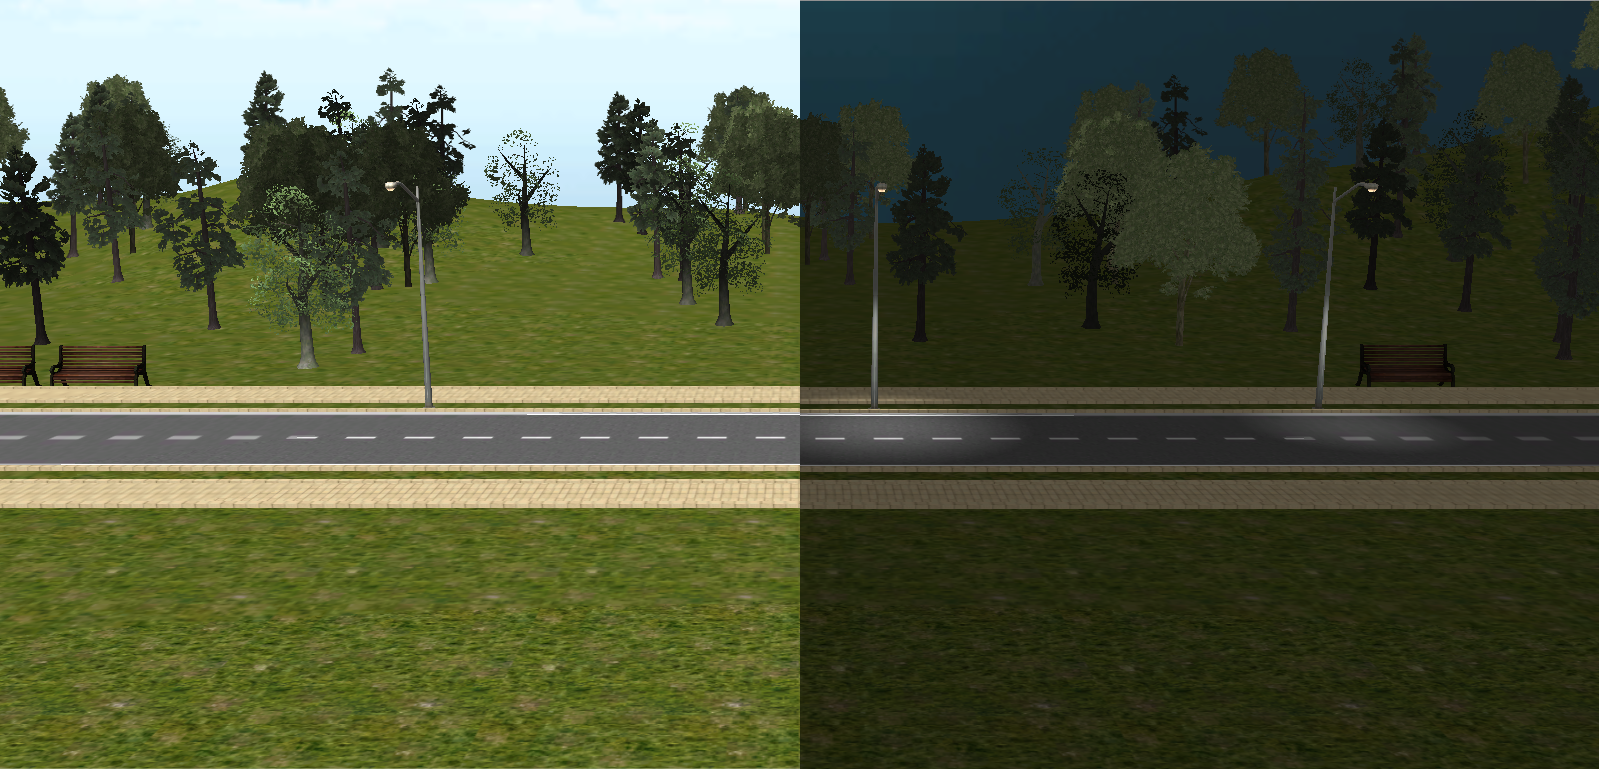
\includegraphics[width=\textwidth]{parkDayNight} 
        \caption{Park scene in Unity developed by Alex St-Onge} 
        \label{fig:park_scene} 
        \end{figure}
		
    \subsection{Rendering the cyclist} 
    
The  base model for the cyclist was imported directly from the asset store.  We wanted a base model that was flexible enough for us to change and adjust to display our purposes.  My partner focused on changing the animation and handling collision avoidance using Unity.  My part involved adding and managing the UV Mapping and texturization of the cyclist to enhance realism.  This involved the combination of smart and manual Blender mapping as described in \cite{UVMap}.  

Generally UV mapping requires the 2D image to be customized for the 3D models UV mapping or visa versa.  Our bike and cyclist model is relatively large compared to the texture sample and the patterns used for the bicycle and clothing components tend to use repeating patterns.  Therefore we took advantage of this applied tileable textures to properly UV mapped components.  We obtained the tileable textures from a free online web resource and followed the similar application process of UV mapping shown by blendtuts \citep{BlendTuts}.  Figure \ref{fig:bikebody} shows how tileable textures were used on multiple bicyclist components.

One of the key issues we came across was due to using someone else?s bicycle model.  Some objects were not separated appropriately within the model.  For example,  the wheel and tire was one object.  Ideally  We restrained from altering the blender model too much because imperfect adjustments caused the UV mapping and texture application problems.  Instead we used custom, manual UV mappings when necessary as seen in Figure \ref{fig:uv_map_wheel}.

\begin{figure}[h]
    \centering
    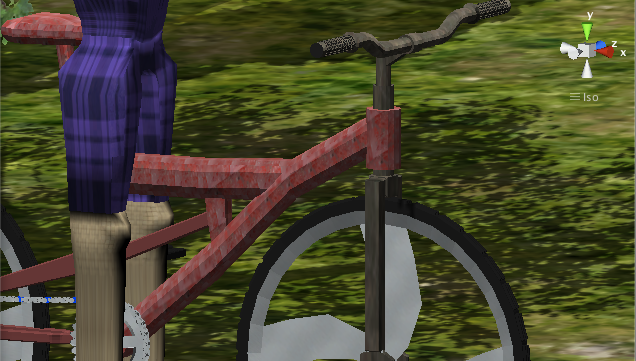
\includegraphics[width=0.75\textwidth]{tileable_bikebody.png}
    \caption{Bike and Clothing tileable texture}
    \label{fig:bikebody}
\end{figure}

\begin{figure}[h]
    \centering
    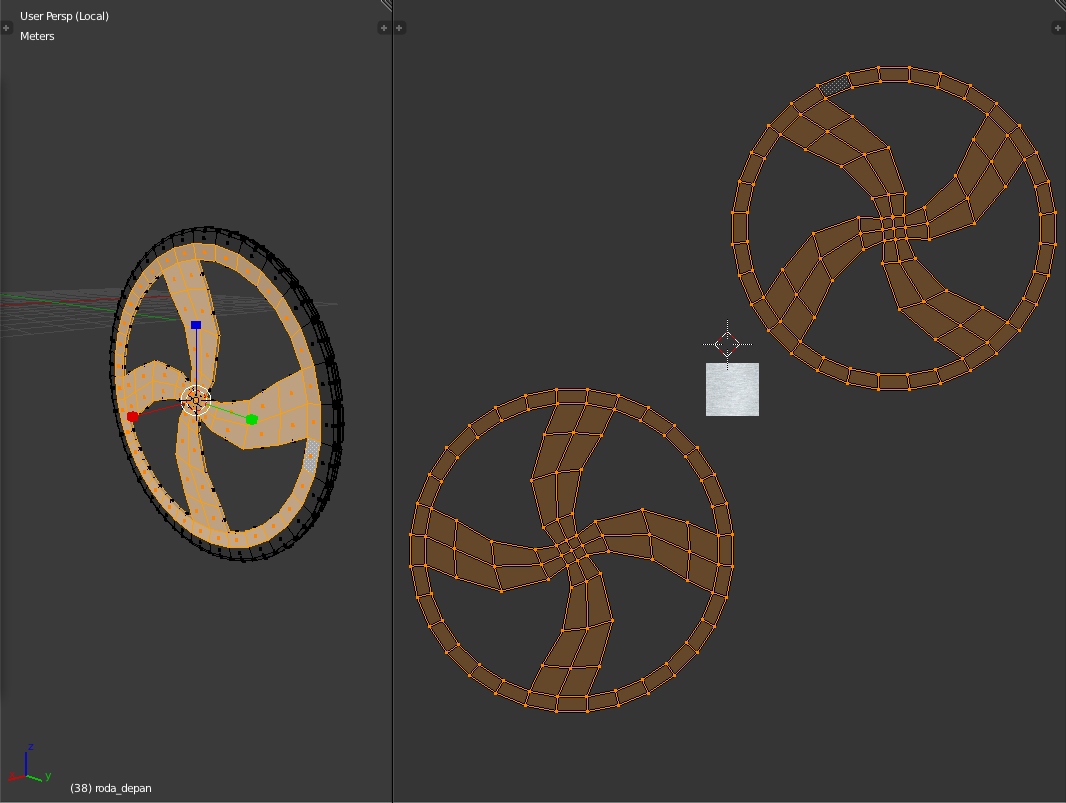
\includegraphics[width=0.75\textwidth]{uv_map_wheel.png}
    \caption{Manual UV mapping of the bicycle wheel}
    \label{fig:uv_map_wheel}
\end{figure}

The bicyclist model constructed of objects the had inconsistent extrusions and cuts leading to complicated UV maps.  The models produced very complex UV maps.  As a result we had to deal with texture segregation as we applied our tilable texture.  Attempting to follow some guidelines presented in \citep{spatfrequency}, we adjust the size and contrast of the texture of each of our models components so that incongruent visual effects are less noticeable in the background scene.  Figure \ref{fig:fullbike} shows that keeping our texture details small relative to the scene?s camera distance to the cyclist allowed us to be able to utilize the same UV mapping and be able to substitute out textures.  

\begin{figure}[h]
    \centering
    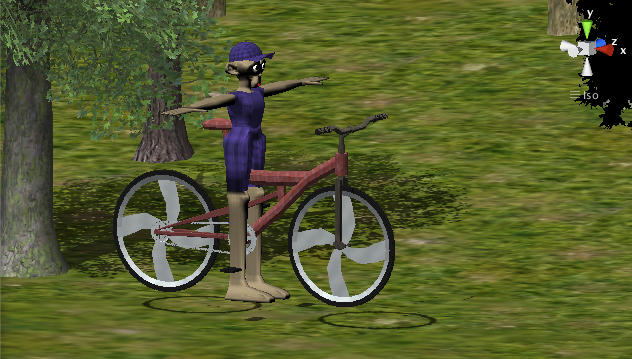
\includegraphics[width=0.75\textwidth]{bike_fullshot.png}
    \caption{Overview of the full default Bicyclist.  Level of texture detail is adequate for the limited user attenuation}
    \label{fig:fullbike}
\end{figure}
		
    \subsection{Creating the Custom Shaders} 
        
        We decided to write our own shaders in order to deal with different types of light sources for particular objects on our cyclist model.   In Unity shaders are written in CG.  	In particular, blocks of code (passes) need to be written for every light source that affects the material. We found with the way our scene was structured there was at 	most two lights on a single object.  Therefore, we wrote two passes for every shader that we created.  This reduced the number of processing resources as more cyclist 	were introduced into the scene.  Figure \ref{fig:bike_under_lights} shows the near optimal result of limiting our shader to just two passes.

	\begin{figure}[h]
   	 \centering
   	 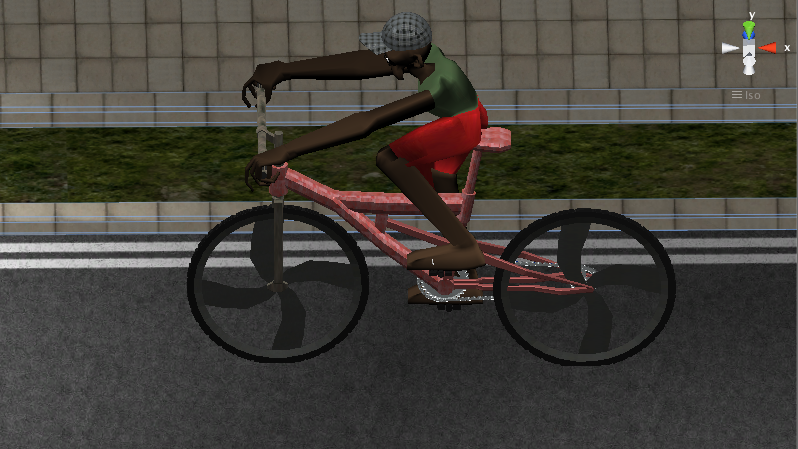
\includegraphics[width=0.75\textwidth]{bike_undertwo_lights.png}
   	 \caption{Bike under two lights.  The bike frame demonstrates how reflection is highlighted on both the front and the back.}
   	 \label{fig:bike_under_lights}
	\end{figure}

	It was essential that we wrote custom shaders for the major types of materials used by our cyclist model.  In CG we had to define input structs that were used to store 	data for per vertex and fragment operations.  Structs allowed us to hold temporary data values of specific types.  
		
        \begin{lstlisting} 
        struct vertexInput{
		float4 vertex : POSITION;
		float3 normal : NORMAL;
		float4 texcoord: TEXCOORD0;
	};
	struct vertexOutput {
		float4 pos : SV_POSITION;
		float4 tex : TEXCOORD0;
		float4 posWorld : TEXCOORD1;
		float3 normalDir : TEXCOORD2;
	};
        \end{lstlisting}		

        All of our shaders dealt with different light sources.  For our metallic and clothing shaders we had to calculate for diffuse and specular reflection.  We defined a unity 		attribute for the shininess of the material. Therefore we did not have to alter the code make metallic materials more reflective.  Instead we just alter an attribute.  		However, we decided to include rim lighting to our metallic materials.  This provides a modest glow effect around our metallic materials while non metallic material has a 	more modest reflection.  
		
        \begin{lstlisting} 
        float3 rimLighting = atten * _LightColor0.rgb * 
        		_RimColor.rgb * saturate(dot(normalDirection, 
		lightDirection)) * pow(rim, _RimPower);
         \end{lstlisting}	
	\begin{figure}[h]
   	 \centering
   	 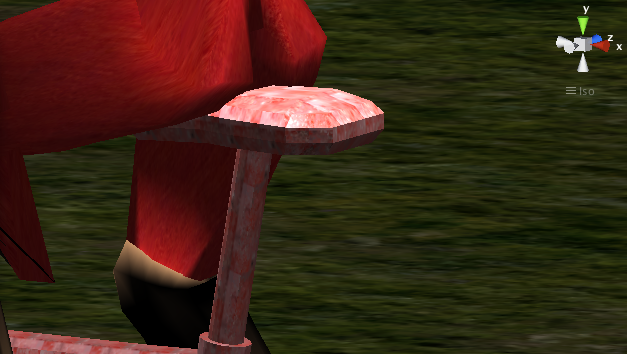
\includegraphics[width=0.75\textwidth]{Glow_effect.png}
   	 \caption{Bike seat unclose that shows the combination of specular and diffuse reflection along with rim lighting.}
   	 \label{fig:bike_seat}
	\end{figure}
	
	All of our shaders work with textures.  Textures are applied and defined as Unity attributes.  This allowed us to dynamically change the texture.  Textures had to be 		scaled and adjusted according to the appropriate shader.  
	
        \begin{lstlisting} 
	float4 tex = tex2D(_MainTex, i.tex.xy * _MainTex_ST.xy 
		* _MainTex_ST.zw);
	\end{lstlisting}		
        
	\subsection{Creating Controls} 
		
One of my primary objectives was to provide a varying levels of detail.  While \citep{peters2011crowds} explores how represent realistic representations of pedestrians.  We looked to apply similar methodology to modeling realistic cyclist scenes.  We wanted to design our tool to be adjustable so we could explore how to make more realistic scenes.  I wanted to have each cyclist to be able to appear realistic and different than the previous cyclist.  I added to the bike generation script allowing the cyclist components to have different textures.  These textures can be defined as unity scene attributes.  

	I created a Unity controller that controls the variability of the cyclist appearance.  My goal was to reduce the amount recognition and recall of similar cyclist in the scene.  	\citep{memory} addresses how effective viewpoints can be when it comes to recognition.  In our situation we wanted to reduce the amount of recognition.  Our camera view is orthogonal to the direction of the cyclist.  Therefore, we had to supplement the higher probability of recognition with higher texture variability and lighting augmentation.	
		
	\subsection{Connecting to Citibike Data} 		
		
	I, along with a team of other KTH students, designed and implemented a framework to help people visualize and analyze data.  One of the key aspects of this 			framework was the ability to make analytics request as REST request.  For the purposes of this project, I implemented a portion of the REST service that provides the 	prevalence of trips between to bike stations.  This prevalence is the ratio of the total number of trips from the start and end stations weighted the by the max number of 	trips from the start station to any other station.  

	I added the ability for Users to control if they wanted to manually control simulated bicycle traffic or connect to the latest aggregated Citibike data within our Unity scene.  	The User Interface is still very young and it was only designed for proof of concept.  In actual analytic practice, we envision the scene to be supplementary to other 		processes.  Specifically, we assumed that the parameters for the traffic simulation would be controlled externally.
		
\section{Challenges} 		
	
We used a bicyclist model that was initially created by someone else.  We found parts of the model were too monolithic.  For example, the bike seat and upper bike 		frame were all one piece.  This made the task of creating UV maps and texturing more difficult.  I was able to separate out the components like the wheel and the tire but in the example of the bike seat, I was unable to separate the components.  Figure \ref{fig:bikebody} and \ref{fig:bike_seat} show the difficulty of object texture separation.

Writing shaders in Unity/CG was not a trivial task and required doing a lot of 3rd party research.  Cg is very susceptible to syntax, type cast, and various other technical bugs.  Eventually, I was able to reduce specular, diffuse, and rim lighting calculation a few lines of code once I figured out the nuances.  

\begin{lstlisting} 
// Lighting
float3 diffuseReflection = atten * _LightColor0.rgb * saturate(
	dot(normalDirection, lightDirection));
float3 specularReflection = diffuseReflection * pow(saturate( 
	dot( reflect( -lightDirection, normalDirection), viewDirection)), 
	 _Shininess);
// Rim lighting
float rim = 1 - saturate(dot(viewDirection, normalDirection));	
float3 rimLighting = atten * _LightColor0.rgb * _RimColor.rgb * 
	saturate(dot(normalDirection, lightDirection)) * pow(rim, 
	_RimPower);
\end{lstlisting} 

In order to dynamically change the texture of components I decided to use tileable textures instead of custom ones. \citep{spatfrequency} describes how local and global  repetition effects viewer cognition.  I wanted to ensure the level of detail was effective enough for the entire cyclist model to look as realistic as possible at the scene's camera position.  At the current scene?s camera distance the temporal locality and the level of detail of the bicycle was deemed suitable for a natural appearance.

Currently, our server houses a database about Citibike bicycle trip data.  We have a record for the starting and ending station of every bike trip within a finite amount of time.  We have to calculate the relative traffic density by normalizing the numbers of trips over maximum number of trips.  Ideally we would like to connect to a live traffic feed of bicycle traffic.  Unfortunately, that kind of data does not currently exist.
		
\section{Conclusion} 
This project allowed us to exercise implementing important graphical shading concepts within a specific context. It also allowed us to build a tool to create background bicycle scenes.  We can alter the speed, traffic density, and variability of the bikes in the scene.  We connect to real data via a REST API.  However, in the future we would like to run scientific trials to assess what is the ideal canonical parameters for a bicyclist scene.  There is also room to connect directly live traffic data.  The current data available 	from \cite{citibike} and similar services are kept as a simple log format.  There were no route data available.  The project was a good exercise and challenge for my partner and I to incorporate multiple facets of Data Analytics and Computer Graphics.
        
        \subsection{Task Matrix}
        \begin{center}
   		\begin{tabular}{ | l | p{5cm} |}
    		\hline
		Task & Team Member  \\ \hline
    		Render background scene & St-Onge \\ \hline
		Render Bicyclist & St-Onge \\ \hline
		Animate Bicycle movement & St-Onge \\ \hline
    		Create scene controls & St-Onge and Hotan \\ \hline
		Bind Bicycle generation to controls & St-Onge \\ \hline
		UV - Mapping and Textures & Hotan \\ \hline
		REST API and Server & Hotan \\ \hline	
		Unity REST Client & Hotan \\ \hline
		Scientific Assessment of Realism & Not Complete \\ \hline	
		Connect to Real time traffic data & Not Complete \\ \hline														
		\end{tabular}
	\end{center}
        
        \subsection{Links}
           
	\begin{itemize}
		\item Demo Video \url{https://www.youtube.com/watch?v=nZhTO4bQLfs}
  		\item Graphics Project Repository: \url{https://github.com/mhotan/DD2323.git}
  		\item REST Server Repository: \url{https://github.com/mhotan/CityBikeDataExplorer.git}
	\end{itemize} 

\bibliographystyle{plainnat}
\bibliography{reference}

\end{document}

